In this chapter we will discuss the implementation on various modules of the \sys\ architecture. We start off by describing all the components we worked on and then explain in detail the parts which are relevant to this thesis.

\section{Parts of the \sys\ Architecture}

We have created multiple modules, each with a different functionality and objective. We list the major modules in the \sys\ architecture below:

\begin{enumerate}
	\item \textbf{Main Controller} - This component manages the flow of data and information among the other components. It reads and cleans the data and manages the training and prediction of the dialogs via the memory network.
	\item \textbf{Data Loader} - This is incharge of reading all the data from files and formatting it in an easy to use way.
	\item \textbf{Data Batcher} - This module takes data from the data loader class and performs any preprocessing and indexing required by the Memory network to use the data for training.
	\item \textbf{Memory Network} - This is the network of the encoder and decoder that both trains and predicts the responses for dialogs given the context and user query.
	\item \textbf{Dynamic Decoder} - This is a built in library of tensorflow that was modified to allow batch decoding and beam search.
	\item \textbf{Attention Mechanism} - This is a built in library of tensorflow that was modified to enable our multi-level attention mechanism.
	\item \textbf{Beam Search} - This is the built in library of tensorflow that was modified to allow constraint decoding and the copy generate mechanism.
	\item \textbf{Evaluator} - This class gives evaluation metric scores on the response predictions by comparing them with the gold examples.
	\item \textbf{Logging} - This component maintains any errors in the code during runtime and allows for automatic deployment of multiple runs. It also generates log files giving detailed explanations of each run.
\end{enumerate}

We depict the interaction between the multiple components in Figure \ref{fig:sys_comp}. Parts in blue have been explained in this thesis. Half colored blocks mean part of the work regarding that component is explained and the rest is not in the scope of this thesis.

\begin{figure}[!ht]
\centering
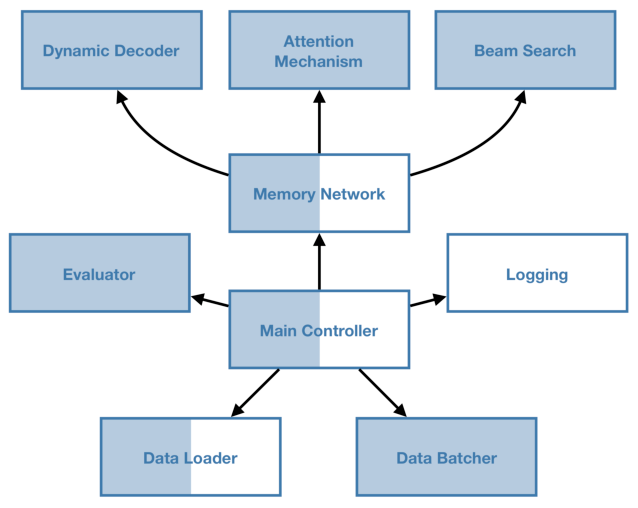
\includegraphics[scale=1.0]{assets/figures/components_orig.pdf}
\caption{Components of the \sys\ system and their interaction.}
\label{fig:sys_comp}
\end{figure}

\noindent\textbf{Main Controller}

This is the main file that we run from the terminal interface. It manages the input parameters that are given by the user and makes sure they are accessible by any another part of the code in other files as well. It is incharge of calling the Data Loader and the Data Batcher to read the data, preprocess, and getting it ready to be fed as input to the main memory network. 

It maintains the train, validation, and test sets separately, each with its different purpose. The validation set is used for early stopping and the state is stored for the best observed validation score using \emph{tf.saver}.

Finally, it is incharge of collecting the responses for each dialog from the model and running the evaluation scripts to get the final metric scores to output to the user. 

For readability of the processing and training, we use the \emph{tqdm} library to easily visualise progress as well as get important information such as average loss and time-per-epoch

\noindent\textbf{Data Loader}

This class is responsible for reading the dialogs from corresponding files (train, validation, and test). It breaks each dialog on each turn into deparate dialogs. Each dialog is further broken into three parts: context, user query, and system response.

\noindent\textbf{Data Batcher} 

The data batcher is responsible for all the preprocessing that needs to be done on the data. Each word has to be replaced with its corresponding index and we have to maintain list of OOV words as well. It removes punctuation and also adds special characters that will aid in training, such as EOS and UNK. All KB associated words are also tagged during the preprocessing which will be important when implementing disentanglement loss.

Further the data batcher is responsible for effectively partitioning the data into batches so that they can be sent into the memory network for training and prediction.

\noindent\textbf{Memory Network}

This is the main \sys\ model containing the entire architecture as discussed in Chapter \ref{chap:approach}. It hosts the multi-hop encoder and the generative, copy-enabled decoder. It is implemented as a class with all the associated hyperparameters as private variables of this class. This enables us to easily store and transport any learned model, as it has all the information needed to run.

The model has two APIs exposed to the Main Controller: \emph{batch\_train} and \emph{batch\_fit}. The first one is responsible to train the weights of the model parameters and implements back-propagation over the whole network after calculating the loss. The gold responses are passed as input to the train API. The second one is responsible for predicting the correct responses, but does not perform any learning of the weights. The only inputs to this API is the current dialog context and the user query.

\noindent\textbf{Dynamic Decoder}

This component was modified from the original Tensorflow decode library. Its objective is to enable batch decoding in which each prediction of each batch element can be of different sizes. We modified it so that at each timestep it combines the generate vocab distribution and the attention distribution. The code listing for this weighted combination is given in Appendix \ref{code:dists}. We also modified the outputs from this library which now also outputs the p\_gen values along with each weighted vocab distribution. This is important for calculating disentanglement loss.

\noindent\textbf{Attention Mechanism}

This component was modified from the original Tensorflow decode library. We changed the way that it computes attention so that it could handle multi-level attention over our multi-level {\sc{BoSs}} memory. We changed the output of its APIs so that they could incorporate the new attention information. The code listing for the new attention mechanism is given in Appendix \ref{code:attn}. We show how to generate sentence level and word level attention seperately and how to combine them.

\noindent\textbf{Beam Search}

The beam search decoder is another built-in library in Tensorflow which we have modified to work with our modified dynamic decoder, attention mechanism, and copy-enabled output generation. The beam width can be any number as required and has been tested to beam width sizes of 64. It also does a weighted generate and attention combination, which now has to be applied onto multiple beams simulataneously, leading to increased complexity.

\noindent\textbf{Evaluator}

This is a script that takes the predicted and the gold responses and performs evaluations of serveral kinds. These evaluated scores are then sent to the main controller which displays them to the user. 

Some metrics evaluated by the evaluator are:
\begin{itemize}
	\item \emph{BLEU Score} - This is a standard metric used on the real-world datasets where exact matches between predicted and gold responses is very rare. Hence BLEU helps to measure degree of closeness of the prediction.
	\item \emph{F1 Score} - This is a combination of Recall and Precision over the predicted KB items in the responses.
	\item \emph{Per-Response Accuracy} - For the fabricated datasets (bAbI) we look for an exact match between predicted and gold. The extent of exact matches is measures via this metric.
	\item \emph{Per-Dialog Accuracy} - This measures how many dialogs had all perfect response predictions for all its turns.
\end{itemize}

\section{Parts of the \sys\-RL Architecture}

There are mainly three main components that have been added to the \sys\ architecture to make \sys -RL. These are listed below.

\begin{enumerate}
	\item \textbf{API Explorer} - This systematically searches the space of APIs and populates the buffer to be used by MAPO.
	\item \textbf{Rewards} - This takes in a particular API as input along with the expected future responses and returns the reward/pseudo-reward.
	\item \textbf{RL-Decoder} - This is the main API generator which we train to learn the ideal policy.
	\item \textbf{Augmented REINFORCE} - This takes in results from both the API explorer populated buffer and the RL-decoder outputs and runs Augmented REINFORCE (MAPO) on top of them.
\end{enumerate}

We observe the interaction between these added components and the previous architecture in Figure \ref{fig:sys_comp_rl}. Below we discuss modifications to previous components and newly added features.

\begin{figure}[t]
\centering
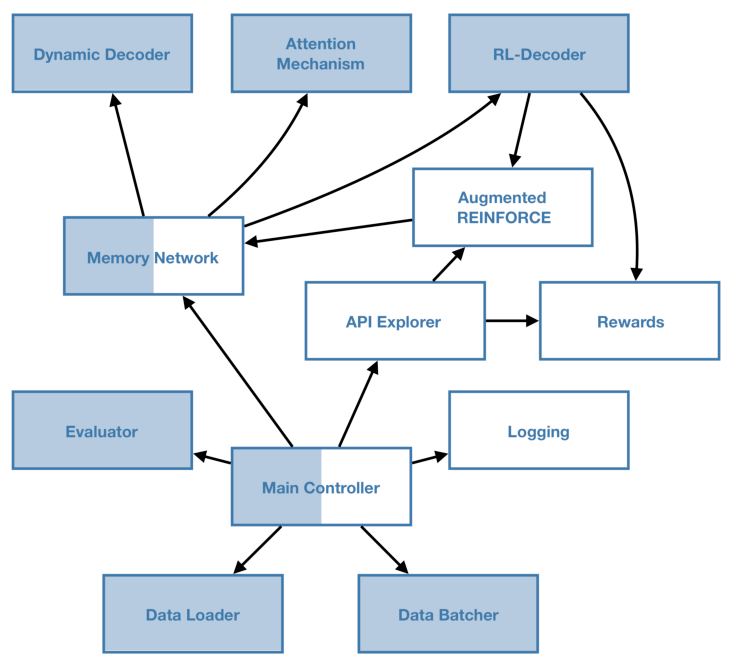
\includegraphics[scale=1.2]{assets/figures/rl_components.pdf}
\caption{The components of the \sys -RL system and their interaction.}
\label{fig:sys_comp_rl}
\end{figure}

\noindent\textbf{Main Controller}

There are several changes that had to be made to the main controller to handle the RL-decoding policy. First, we implemented a phase-wise training to help enable the RL-decoder and the response model to train independently. In this phase we have 4 phases:
\begin{enumerate}
	\item \textbf{Phase 1} : This trains the response deocder only for dialogs that occur before any API is made.
	\item \textbf{Phase 2} : This phase adds in the training for the RL-decoder. This is only used in case we use a shared embedding space for encoding the context for the response deocder and RL-decoder. If they use different embeddings, then Phase 2 can be directly merged with Phase 1.
	\item \textbf{Phase 3} : In this phase we can now start training the system on responses after the API call has been made. We include the results retrieved by the RL-decoder in Phase 2.
	\item \textbf{Phase 4} : This phase calculates the actual reward based on the responses innn Phase 3 and retrains the RL-decoder accordinly. This reward actually measures how well the system was able to train on the retrieved results and will be able to capture the effects of how the results are stored in memory, like sorting based on a field.
\end{enumerate}

These phases are run one after the other and more phases are activated after the previous phases near convergence. For example we start off with just Phase 1 and after it converges we now run Phase 1 and 2 together.

\noindent\textbf{Memory Network}

We added three main APIs in the memory network to enable the RL-decoder. 

\begin{itemize}
	\item \emph{api\_predict} will attempt to predict good API responses via the RL-decoder policy and utilises beam search to get a large set predictions.
	\item \emph{api\_train} takes in APIs and their rewards and then implements the augmented REINFORCE algorithm
	\item \emph{api\_prob} takes in an API and returns the probability of generating that API with the current policy.
\end{itemize}

\noindent\textbf{RL-Decoder}

The RL-decoder takes in the encoded state as the inital state. It maintains a time variable which corresponds to the current time step of the decoder. This time variable is sent through a position embedding and is then sent as input to the decoder. We set the next state of the decoder as the inital state so that we break the sequential behavior as required. This decoder uses the dynamic decoder with beam search to decode and attends over the input context via the attention wrapper.
